% !TEX root =  paper.tex
\section{DigiTaps}
\label{sec:digitaps}

Since the preliminary evaluation of DigiTaps shows promising results, a more rigorous study is needed to evaluate the gestures more thoroughly. We adopted the user study model presented in \cite{Henze:2011} to conduct our user study. We developed DigiTaps Game, a platform for cøonducting number entry method user studies in the large.
\par
The Espresso and the Cappuccino methods have been evaluated in a lab study as presented in \cite{Azenkot:2013}. However, the lab studies does not reflect the actual use of the gestures, so we want to design user studies that simulate real world use of the gestures. We assume that number entry speed is the prominent factor for the \textit{real world use}, so we decide to incentivize users to enter the numbers as fast as possible by designing DigiTaps as a game.
\par
In addition to simulating real world use, we gather data from the players by keeping track of the gestures they perform. We save the data in our database to do further analysis on the data. To gather as much data as possible, DigiTaps is distribute the game via the Apple App Store.

\subsection{Flow of DigiTaps}
% describes the game states
The first screen shown to the player after launching DigiTaps is the main menu of the game as (see Figure \ref{startscreen}). This screen consists of three choices for the player to choose
  \begin{enumerate*}[(1) ]
    \item Tutorial, 
    \item Start Game, 
    \item Leaderboard.
  \end{enumerate*}
  Selecting different button leads to different modes of DigiTaps and leads to different screens that the player visits.
  
\begin{figure}[ht!]
  \centering
  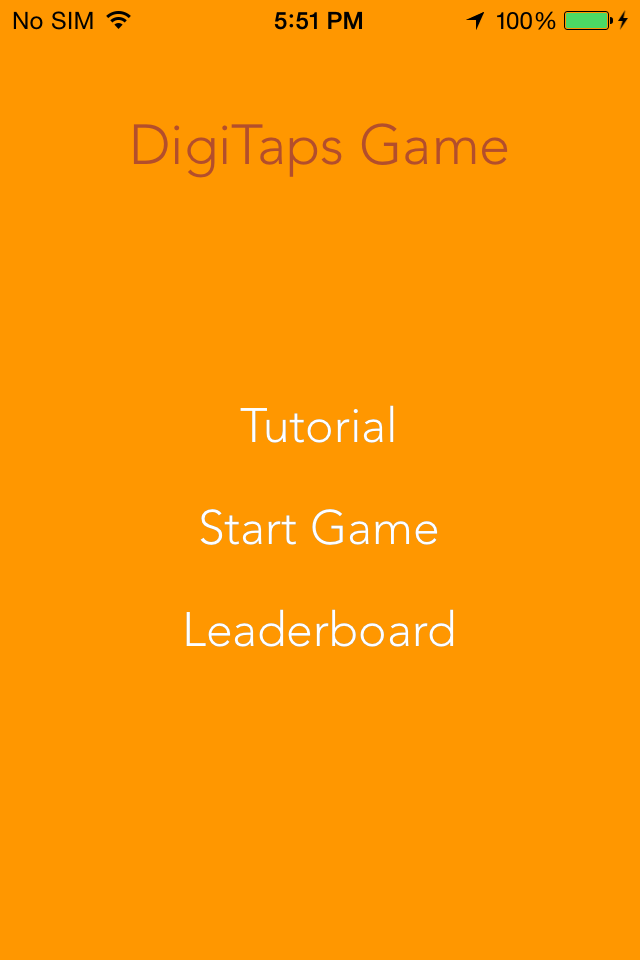
\includegraphics[width=0.5\textwidth]{figures/start.png}
  \caption{Main menu and the first screen of DigiTaps}
  \label{startscreen}
\end{figure}

\subsubsection{Tutorial}
    We provide some tutorials for the players before jumping into the game. Each of the tutorial consists of two main parts the description of the tutorial and the practice mode for the tutorial. There are three tutorials total. The first tutorial is the overall description of the game. It describes the main gestures such as long-press to submit the number. The two other tutorials describe the DigiTaps method. There is a table at the bottom of each DigiTaps method tutorial. The practice screen is an empty screen for the player the play around with the gestures they learned. The screen gives the user feedback on the action the player just perform. For example, if the player tap the screen with three fingers, the screen shows that it is a three-finger tap (see the rightmost state in figure \ref{tutorial}).

\begin{figure}[ht!]
  \centering
  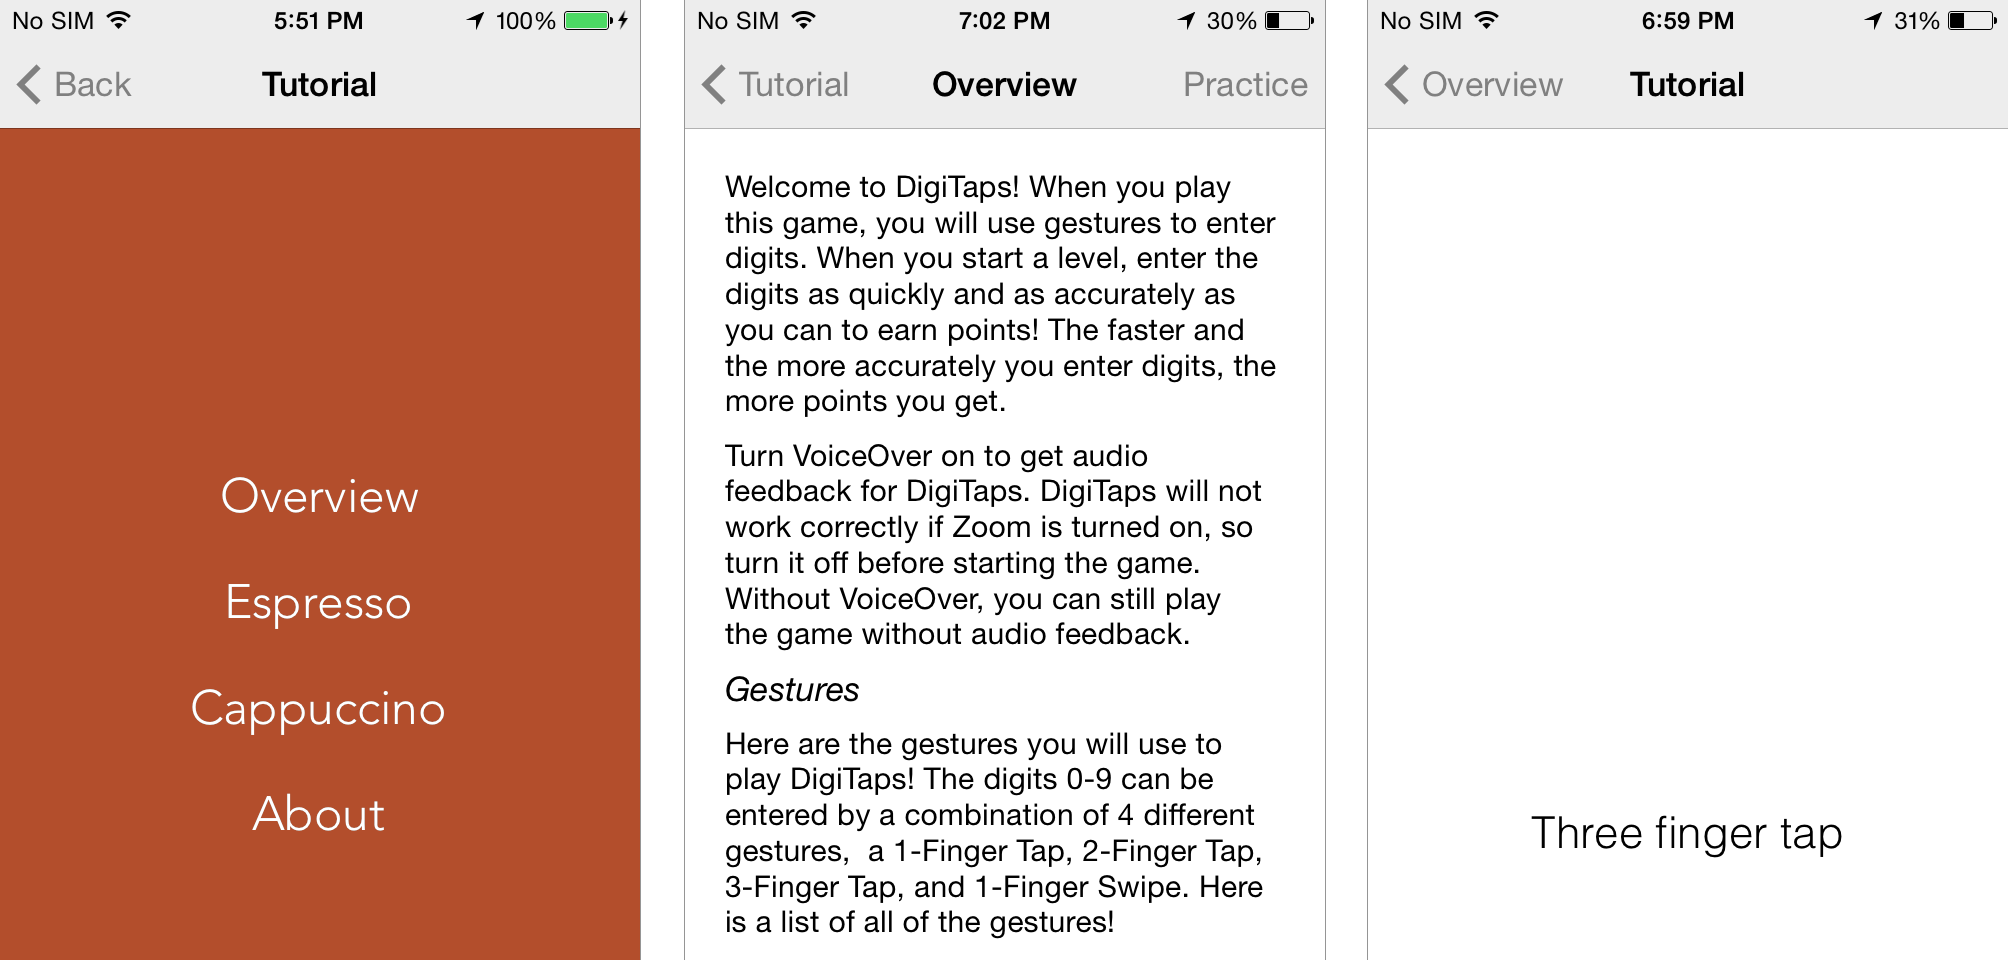
\includegraphics[width=1.0\textwidth]{figures/tutorial.png}
  \caption{The state on the left shows the options the player can choose to learn about. The state in the middle is an example of a tutorial page where descriptions are provided. The state on the right is an example of a practice screen.}
  \label{tutorial}
\end{figure}

\subsubsection{Game Play}
    \begin{enumerate*}[(1) ]
      \item a DigiTaps method selection screen, 
      \item a level selection screen, 
      \item a game play screen, and
      \item a summary screen.
    \end{enumerate*}
    At the method selection screen, DigiTaps lets the player choose either the Espresso method or the Cappuccino method, in which the player is going to use that method to play the game. After the method has been chosen, the player can choose a level to start playing the game, indicated by the red arrow in figure \ref{gameplay} from the top row to the leftmost state on the second row.
\par    
At this point, the game play screen slides in and show the first number to the player (see the leftmost state of the second row in figure \ref{gameplay}). The player performs the gesture to enter the number shown on the screen. To submit the number, the player has to tap and hold that finger on screen with one finger until the ring or the buzz sound occurs. This means that the number has been submitted and DigiTaps advances to the next number. The player has to enter 10 numbers per level and the number of digits per number varies based on the level. The numbers starts with 3 digits per number at level 1 and it increases by one digit at each level. At the last level, level 5, each number is 7 digits long.
\par
After entering all the numbers required, the summary screen appears. The summary screens provides the player's performance on that level. The information includes the points earned, the accuracy and the average time per digit. On this screen, the player has the option to advance to the next level, replay the same level or quit to the start menu as (see the last state of figure \ref{gameplay}).

\begin{figure}[ht!]
  \centering
  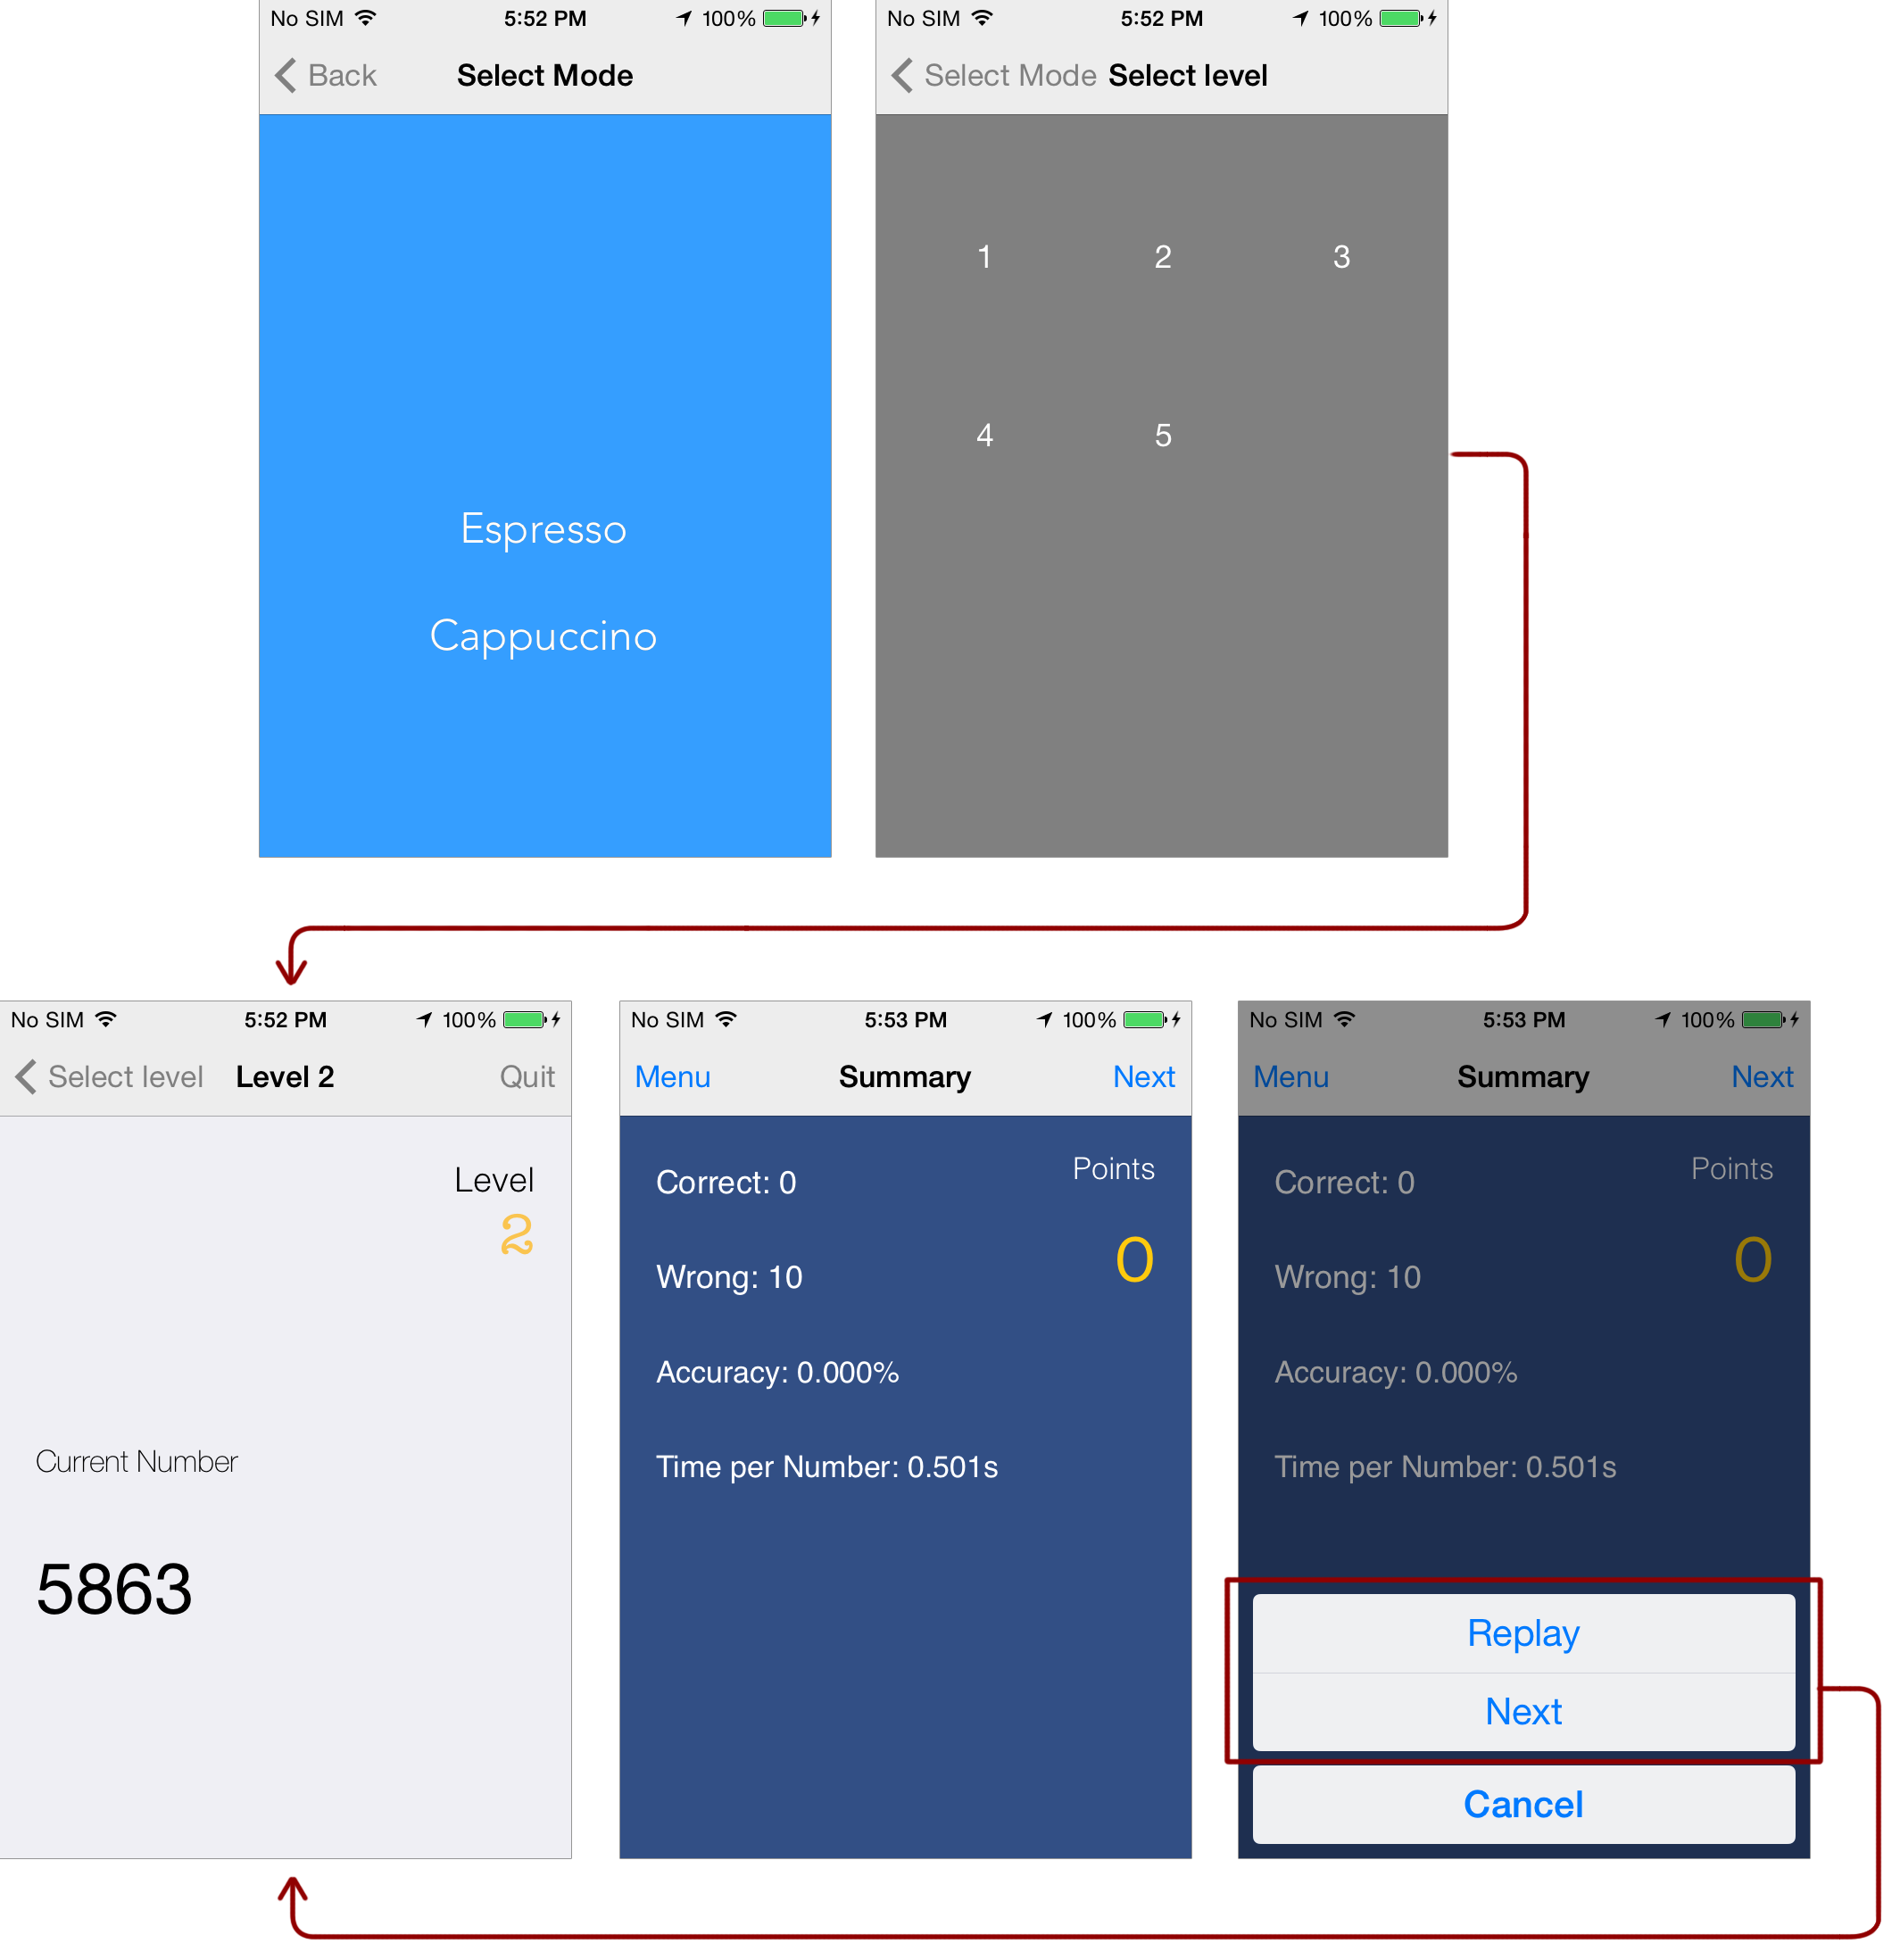
\includegraphics[width=1.0\textwidth]{figures/gameplay.png}
  \caption{Shows the state diagram of DigiTaps gameplay mode.}
  \label{gameplay}
\end{figure}
    
\subsubsection{Leaderboard}
    To provide the players with competition, we include Apple's leaderboard into DigiTaps. The leaderboard ranks the player's score with other players around the world who uses Apple's Game Center. Players are being ranked with respect to their scores they achieved in the game (see figure \ref{leaderboard}).
    
\begin{figure}[h!]
  \centering
  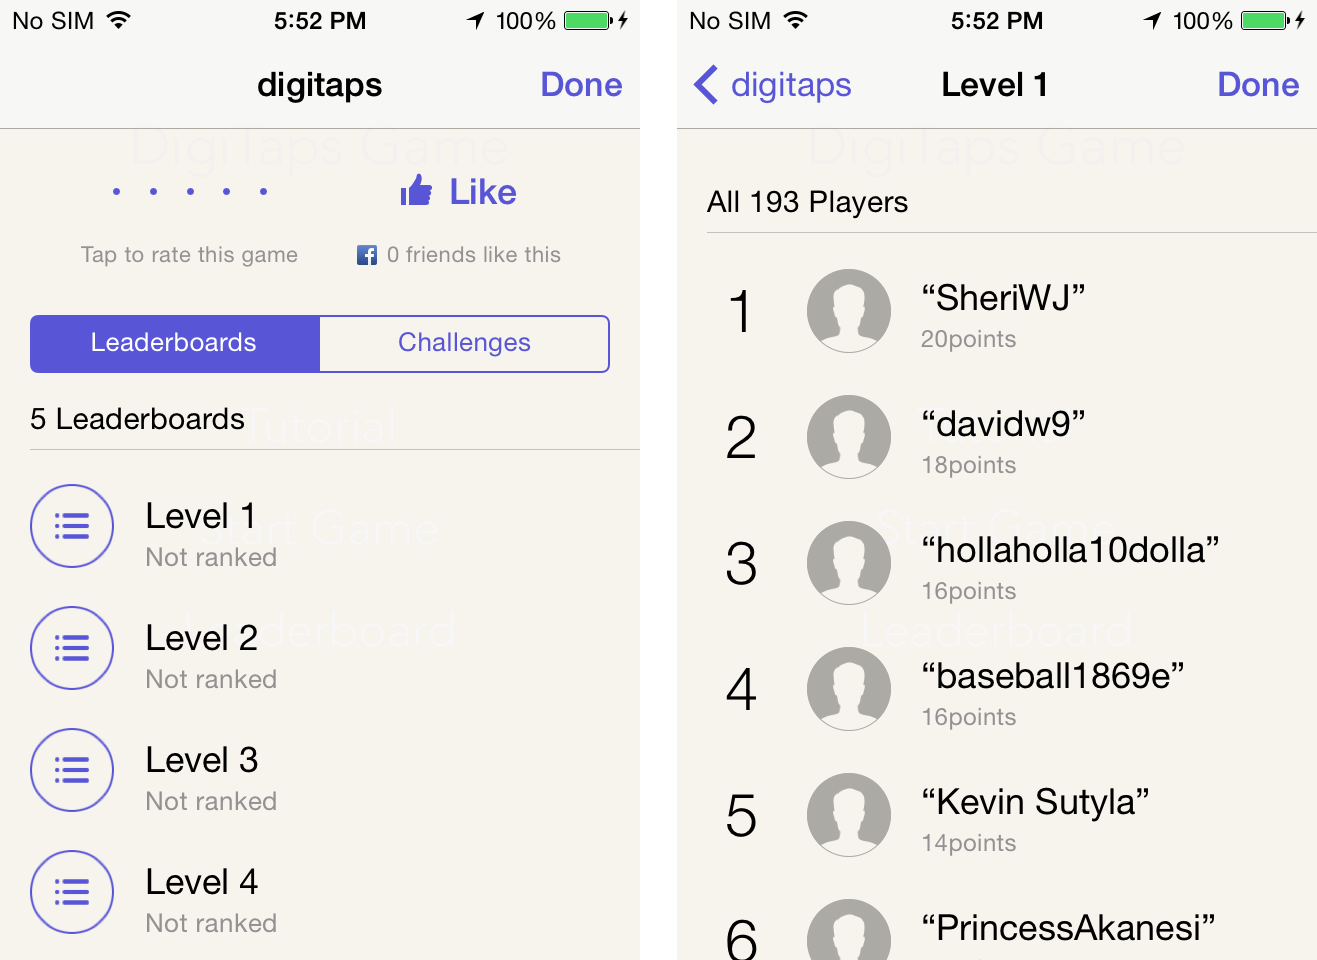
\includegraphics[width=1.0\textwidth]{figures/leaderboard.png}
  \caption{The state on the left shows the leaderboard of each level. The state on the right shows the rankings of the first six places for level 1 with their respective points.}
  \label{leaderboard}
\end{figure}

\subsection{Interaction Gestures}
In addition to the DigiTaps gestures described in the DigiTaps code, DigiTaps has two other gestures for players to interact with the game. The first gesture is two-finger swipe in any direction. This gesture does two main action in the game. First, it acts as the backspace gesture. We have to use two-finger instead of one because the DigiTaps gestures have already used one-finger swipe in any direction. It also acts as the repeat gesture. When the player starts entering numbers, the number initially shown on the screen disappears. To see the given number again, the player has to delete all the digits inputted using the backspace gesture and do an additional backspace gesture to make the given number appear.
\par
The second special gesture is the long-press gesture. This gesture is used for advancing to the next number in the level or if there is no more number on that level, this gesture takes the player to the summary screen. When the player finishes inputting the given number, the player holds one-finger down on the screen until there is a bell ring or a buzz sound from DigiTaps. The sound indicates that the game has advanced to either the next number or the summary screen. The bell sound indicates a correct attempt and the buzz sound indicates a failed attempt.

\subsection{Data Collection}
In order to conduct the user study, we collect two different information from the players. We collect the players or the study participant's demographics. This includes the player's age, gender, experience with accessibility in iOS. Each player is uniquely identify with an identification number. However, we cannot trace back to who the actual player was. This identifier is used to match the player to the other information of this player that collected.
\par
In addition to the demographics, we collect the touch events that the player performs in the game. Every touch event is recorded. This includes touch-down, touch-move, and touch-up events. In each of these touch events, we record the number of fingers on that touch event, the location of the touches and many other information. Furthermore, we recorded the state of the game such as when the game starts, the level finishes, the number is inputted, and some other game states.
\par
Using the information collected, we can gain some insight on how the players behave in the game. More important, we can evaluate the gestures with the data gathered to see which of the gestures performs better.